\documentclass[conference,9pt]{IEEEtran}
\usepackage{xcolor}
\usepackage{cite}
\usepackage{epsfig}
\usepackage{amssymb}
\usepackage{amsmath}
\usepackage{graphicx}
\graphicspath{ {./} }

\begin{document}
\title{Practical 4a}

\author{
\IEEEauthorblockN{Albert Acebron}
\IEEEauthorblockA{NIU: 1458626}
}

\maketitle
\begin{abstract}
In this practical we will implement the LMS algorithm and test it against a noisy signal.
\end{abstract}

\section{Questions}

\subsection{Question 1}
$\mu$ is fundamentally a parameter that is tied to the size of the step taken on every iteration of the algorithm. That is, once the algorithm computes the gradient and knows what's the best direction to move forward to reach the minimum, it must also choose how big of a movement in that direction it should make, and this is determined by $\mu$ (along with how steep the gradient is at that point).

This means that, on one side, the smaller $\mu$ is, the smaller will be the steps that the algorithm takes to reach the local minimum, which will increase the total number of steps taken by the algorithm, thus making it slower. Furthermore, it's also possible that a small step size makes the algorithm get stuck in a small local minimum or, if a fixed amount of steps is used, that it is unable to reach a minimum before the algorithm finishes. On top of that, in circustances where the filter coefficients have to keep changing to adapt to changes in the environment or input signals, if the step size is too low the filter won't be able to change quickly enough to properly adapt.

On the other side, if the value of $\mu$ is too high we might end up in a situation where we overshoot the minimum and end up in the other side, which could make our algorithm slower (since we are constantly overshooting the minimum instead of closely following the steepest descent) or might even end up preventing our algorithm from converging.

In conclusion, we want to pick a value for it that it's not too small nor too big, in order to make our algorithm finish in the lowest time while also making sure it converges.

In data science it's common to vary the value of this parameter during optimization\footnote{Source: https://en.wikipedia.org/wiki/Learning\_rate}, but here we'll just set some bounds and pick a value that ensures convergence.

\subsection{Question 2}

Given equation 1.5, which lets us calculate the new error after each consecutive step:
$$e'(n)=e(n)(1-\mu x_n^H x_n)$$

We can assert that if we want $e(n)$ to eventually converge to 0 we must make sure that the following condition is met:
$$|1-\mu x_n^H x_n|<1$$

This is because if this doesn't hold we would end up in situations where the error after applying a step is equal or larger than the one before applying the step, which means that we wouldn't be able to minimize it.

Now, if we develop the expression further, we get that:
$$0 < \mu x_n^H x_n < 1$$

And if we unroll $x_n^H x_n$ we would see how it's just a sum of multiplications between an number and it's conjugate, which hold the condition $a\cdot a*>0$, therefore $x_n^H x_n > 0$, which means that to meet the first condition two conditions must be met:
$$0 < \mu$$
$$\mu < \dfrac{1}{x_n^H x_n}$$

Finally we can compute the value of $x_n^H x_n$ with:
\begin{verbatim}
  conj(entrada')*entrada
\end{verbatim}

And we will get a result of 3.8887e+13, thus $\mu$ will need to be contained in:

$$0<\mu <\dfrac{1}{3.8887\cdot 10^{13}}=2.5716\cdot 10^{-14}$$

\subsection{Question 3}
Initially I implemented a simple version of the algorithm:
\begin{verbatim}
function [H, y, e] = algoritmeLMS(d, x, P, mu)
  iterations = P:length(x);
  H=zeros(P, length(x)-P+1);
  first = -min(iterations);
  for j=iterations
    index=first+j+1;
    xn= x(j-P+1:j);
    y(index) = H(:, index)'*xn;
    e(index)=d(j)-y(index);
    H(:, index+1)=H(:, index)+mu*xn*conj(e(index));
  end
end
\end{verbatim}

But when applied to the signal, the extracted sound (equivalent to the error inside the algorithm) turned out to be very noisy in the beginning. I believe this is caused by the fact that the filter coefficients are all initialized to 0, which makes it perform badly until it has gone through a few samples and optimized itself.

To prevent this noisyness, I added another iteration of the algorithm where the last filter coefficients are used as the initialized parameters of the first filter, which succeeded in making the initial filter better and it reduced the initial noise to barely anything, thus improving the result.
\begin{verbatim}
function [H, y, e] = algoritmeLMS(d, x, P, mu)
  iterations = P:length(x);
  H=zeros(P, length(x)-P+1);
  first = -min(iterations);
  for k=1:2
    for j=iterations
      index=first+j+1;
      xn= x(j-P+1:j);
      y(index) = H(:, index)'*xn;
      e(index)=d(j)-y(index);
      H(:, index+1)=H(:, index)+mu*xn*conj(e(index));
    end
    H(:, 1) = H(:, first+max(iterations));
  end
end
\end{verbatim}

\subsection{Question 4}
To recover our sound we'll apply our algorithm and then play the error signal:
\begin{verbatim}
  [H, y, e]=algoritmeLMS(referencia, 
    entrada, 100, 2e-11);
  sound(e, Fs);
\end{verbatim}

\subsection{Value of $\mu$}

Note that the $\mu$ that we've used is outside the convergence range calculated on question 2. This is because, after trying experimentally with multiple posssible values of $\mu$, we achieved the best results with values close to $10^{-11}$, whereas the values contained in our convergency range didn't work well.

This is because smaller step sizes don't manage to reach the minimum within the number of iterations we are using in our algorithm ($2|samples|$), as all movements are very small\footnote{I've verified this experimentally by increasing the number of iterations of the algorithm and checking that even with a small $\mu$ it works fine}, whereas with larger steps the minimum is reached but, because these are outside the convergency range, it's likely that we don't end up in the absolute minimum and instead end up in it's surroundings (and if the step size is too large we could end up overshooting our minimum completely, but this doesn't happen for values around $\mu=10^{-11}$).

Overall, this can be fixed by increasing the total number of iterations of the algorithm from 2 to 20 (in the case of using $\mu=2\cdot 10^{-14}$, if we were to use a smaller value we'd need to increase it even further), which can be done by changing this line:
\begin{verbatim}
  for k=1:2
\end{verbatim}

to this one:
\begin{verbatim}
  for k=1:20
\end{verbatim}

After making this change we can apply the algorithm with $\mu=2\cdot 10^{-14}$ and it will work fine (theoretically the end results should also be better, but I can't tell the difference in terms of sound). All in all, this is a classical example of a computation tradeoff, where if we spend more computation power we can guarantee convergency and make sure we reach the minimum.

\subsection{Number of filter coefficients}

The number of coefficients of the filter was picked through the following steps:

1. Initially pick a random number

2. Apply the algorithm and check that the sound works fine

3. Plot the coefficients to make sure we are not clipping part of the filter.

In this case, looking at the plot of the filter it became clear that only 30 values or so are used for it, as the rest are set to 0 (see plot in question 6), so it's quite clear that with 100 coefficient there is no clipping.

It would be possible to make this number smaller, which would decrease the computation power required for the algorithm, but right now the computations don't take much time so there's no need to do that.

\subsection{Question 5}
It's the opening of Breaking Bad.

\subsection{Question 6}
We can plot the coefficients with the following code:
\begin{verbatim}
  stem(H(:, length(H)))
\end{verbatim}

Which results in:

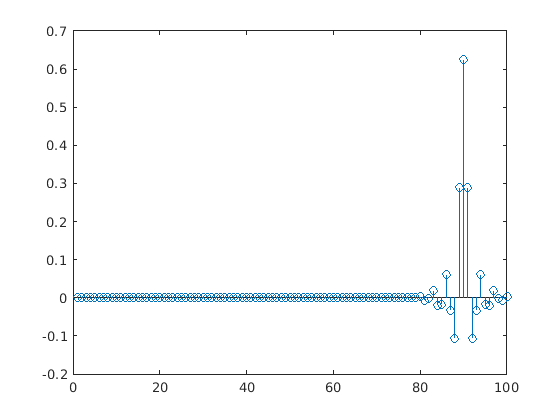
\includegraphics[scale=0.6]{coef.png}

If we were to re-compute the filter using $P=25$, we'd get the following plot instead:

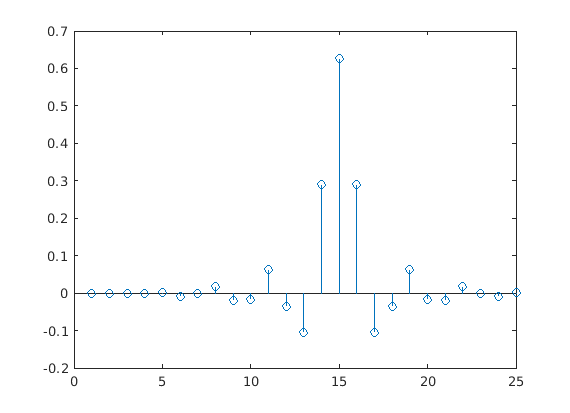
\includegraphics[scale=0.6]{coef25.png}

Note that these coefficients have been obtained from the second algorithm provided, the one that uses two iterations to improve the initial filter estimation.

\end{document}


